\documentclass[AMA,STIX1COL,]{WileyNJD-v2}


% Pandoc citation processing


\articletype{Research article}

\received{2021-01-01}

\revised{2021-02-01}

\accepted{2021-03-01}

\raggedbottom

\providecommand{\tightlist}{%
  \setlength{\itemsep}{0pt}\setlength{\parskip}{0pt}}

\begin{document}

\title{Spike-and-Slab Generalized Additive Models and Fast Algorithms
for High-Dimensional Data}

\author[a]{Boyi Guo*}
\author[a]{Nengjun Yi}

\authormark{Guo and Yi}

\address[a]{Department of Biostatistics, University of Alabama at
Birmingham, Birmingham, USA}

\corres{*Corresponding author name, This is sample corresponding
address. \email{xxx@uab}}

\presentaddress{This is sample for present address text this is sample
for present address text}

\abstract{Spike-and-slab priors have been extensively studied for
variable selection, and recently been extended to function selection in
generalized additive models (GAMs). Most of the previous works on
fitting spike-and-slab GAM relies on Markov chain Monte Carlo (MCMC)
algorithms to identify the promising subsets of functions. The
computational burden of MCMC makes these models less feasible,
especially in high-dimensional setting. Besides, most of the current
spike-and-slab GAM consider an ``all-in-all-out'' approach for function
selection, rendering less flexibility to answer if non-linear effects
are necessary in the model. We propose Bayesian hierarchical generalized
additive models for function selection and prediction. The proposed
models employ spike-and-slab priors, mixture normal and mixture double
exponential, for smooth and sparse solution. Two EM based algorithms,
EM-IWLS and EM-Coordinate Descent, are developed for accelerated
computation. Simulation studies and real data analysis demonstrated
improved performance against the state-of-art models, mgcv and COSSO.
The software implementation of the proposed methods is freely available
via the R package BHAM.}

\keywords{Spike-and-Slab Priors; High-Dimensional Data; Generalized
Additive Models; EM-IWLS; EM-Coordinate Decent}

\maketitle

\newcommand{\bs}[1]{\boldsymbol{#1}}

\hypertarget{introduction}{%
\section{Introduction}\label{introduction}}

Nonlinear effect modeling has long history. Early work of GAMs can date
back to 1979 when \citet{Cleveland1979} proposed local smoothing for
bivariate analysis. Since then, many mathematical and statistical models
has been proposed, see xxx\footnote{TODO: insert an review citation}.
With recent advancement of computing technology, many machine learning
algorithms that is computationally intensive start to gainmuch
popularity in outcome prediction when non-linear effects assumed. Such
models generally have improved prediction accuracy over classic
statistical models, but have a fatal flaw, lack of transparency and
interpretability. The primary objective of biomedical studies is to
understand the etiology of diseases, which requires not only the
knowledge if a biomarker is predictive of the disease, but also how the
biomarker cause the disease. ``Black box'' models could less likely to
be helpful.

As a balance between interpretability and model flexibility,
semi-parametric and non-parametric regression models are studied. Among
those, generalized additive model (GAM) proposed in the seminal work of
\citet{Hastie1987} gains the most popularity thanks to its flexibility
and easiness to incorporate many different smoothing functions. A
response variable, \(Y\), that is assumed to follow some exponential
family distribution \(EF(\mu. \phi)\), can be expressed as the summation
of smooth functions of a given \(p\)-dimensional vector of covariates
\(\boldsymbol{x}\), written as \[
E(Y|\boldsymbol{x}) = g^{-1}(a + \sum\limits^p_{j=1}f_j(x_j)),\qquad E[f_j(x_j)] = 0.
\] where \(g^{-1}\) is the inverse function of a smooth monotonic link
function. GAM solves the model fitting problem for many distributional
outcomes, such as Poisson, binomial, gamma and normal models. In the
same article, @\citet{Hastie1987} proposed the backfitting algorithm
that estimates each smooth function of an additive model iteratively
using partial residuals. The backfitting algorithm is compatible with
almost any smoothing or modeling technique to be used as the
nonparametric components. However, it is unclear how to estimate the
degree of smoothness when necessary, for example for smoothing splines.
The computation cost for cross-validating the smooth parameters can be
expensive. \citet[PP.318-320]{Wood2017} provides more discussion on the
problem.

In many area of modern biomedical research, dealing with
high-dimensional data, also known as \(p >> n\) problem, is common, for
example sequencing data analysis, electric health record data analysis.
Many statistical models have been proposed for such problem, for
example, penalized models and Bayesian hierarchical models. However, up
to this point, most efforts of methodology development focus on modeling
linear effect in high dimensional setting. It is still not clear what is
the best practice on how to model non-linear effects in high-dimensional
setting.

Similar to expanding classic models to high-dimensional models,
expanding the GAM framework for high-dimensional applications is not a
trivial task. The difficulties mainly come in two-fold: grouping nature
of the basis functions, and the balance between spline smoothness and
variable sparsity. For GAM models, a smoothing function is consists of
multiple basis functions. The basis functions of a variable is
inherently related. The grouping structure should be properly taken care
of for accurate estimation. Moreover, shrinkage is previously used
solely for sparsity of the model in high dimensional regression models,
or smoothness in GAMs. How to organically combine the two together
remains as a troubling question.

To the best of our knowledge, there are few GAM models proposed for high
dimensional application. In common practice, model matrix of spline
terms are generated using base functions of preference, and then feed to
a penalized model. Without proper handle of the grouping nature of bases
functions, the estimation of the smooth function is less accurate.
\citet{Bai2020Spline} shows inferior performance of such practice
compared to using an ad hoc high-dimensional additive model. Among the
specialized high-dimensional spline methods, \citet{Ravikumar2009}
extended the original backfitting algorithm \citep{Hastie1987} to
accommodate the high-dimensional setting. The sparsity and smoothness
was handled separately with a soft threshold. The authors also
demonstrated its similarity to Group Lasso. \citet{Meier2009} proposed
an a sparsity-smoothness penalty,

\[
J(f_j) = \lambda_1 \sqrt{||f_j||^2_n + \lambda_2 \int(f^{''}_j(x))^2dx},
\] which can re-formulated as a group lasso problem as well. However,
the model can not estimate the smoothness of the spline functions
correctly, as the smoothness of all spline models are controlled by the
lambda\_2. The inflexible of the model creates problems in prediction.

From the Bayesian perspective, recent works that expands to the
high-dimensional settings includes \citet{Scheipl2012} and
\citet{Bai2020Spline}. \citet{Scheipl2012} proposed an new
spike-and-slab structure prior, normal-mixture-of-inverse gamma for
semi-parametric regression using MCMC. The normal-mixture-of-inverse
gamma prior is mixture of t-distribution with an additional coefficients
mixing vector, where the vector follows a mixture of two Gaussian
distribution. \citet{Bai2020Spline} proposed an novel high dimensional
Bayesian GAM using the spike-and-slab group lasso prior. An fast fitting
EM-based algorithm is proposed. Asymptotic theory, such as posterior
contraction rates and model selection consistency are proved. Even
though, the algorithm is flexible to cover many non-Gaussian family in a
high dimensional setting, the proposed method didn't address uncertainty
quantification, i.e.~calculating credible intervals etc. However, most
of these Bayesian GAMs still suffer a common problem, computation cost.
These Bayesian GAMs uses MCMC to estimate the posterior distribution,
which would create an intense computation load.

In this article, we aim to address the challenges of non-linear signal
modeling in high-dimensional application using Bayesian Hierarchical
model. Specifically, we will propose a new Bayesian spike-and-slab prior
for the generalized additive models and Cox spline models. The
contribution of the proposed prior comes in two-fold: 1) it supports
simultaneous variable selection and function selection; 2) it provides
robust estimation and prediction for the coefficients and outcomes. As
previously described, simultaneous variable selection and its functional
form selection is not a trivial problem. Nevertheless, the Bayesian
spike-and-slab prior is a perfect solution to the problem, as the latent
binary indicator can be used to for variable selection and the spike and
slab densities are used to adaptive adjust the smoothness of the spline
function. Moreover, compared to currently available Bayesian spline
models which mostly conduct a `all-in-all-out' strategy, i.e.~either
including a non-linear form of a variable or excluding the variable
completely, we offer a more flexible solution, rending one of three
possibilities: no effect of a predictor, only linear effect of a
predictor, or non-linear effect. This simplifies the process of
determining what effect a predictor have on the outcome, without
involving hypothesis testing where the degree of freedom for non-linear
effect is complicated to estimate due to the shrinkage. Moreover, out
model inherent the the robust estimation from Bayesian models. Lastly,
The third aim of the dissertation work will focus on the software
implementation of the proposed models and algorithms. We will implement
the proposed models and algorithms in one of the most commonly used
statistical computing environment R. Ancillary functions will be
provided in assistance to model diagnostic, interpretation and graphing.
The R implementation of the Bayesian hierarchical additive model is
available via a freely available R package, BHAM at
(\url{https://github.com/boyiguo1/BHAM}){[}\url{https://github.com/boyiguo1/BHAM}{]}.

The rest of the paper are arranged as the followings: in Chapter 2 we
demonstrate the Bayesian Hierarchical generalized additive model, where
we provide the setup of the proposed model and two fast-fitting
algorithms. In Chapter 3, we Application to real-world datasets
demonstrates the usefulness of the proposed methodologies in Chpater 4.
Conclusion and discussions are made in Chapter 5.

\hypertarget{spike-and-slab-additive-model}{%
\section{Spike-and-slab Additive
Model}\label{spike-and-slab-additive-model}}

Following the notation in the previous section \ref{Notation}, suppose
we have the model matrix \(\boldsymbol{X}\) derived from spline
functions of choice \(h_j, j = 1, \dots, p.\) for the \(p\) covariates
that are modeled nonparametrically, the total dimension of
\(\boldsymbol{X}\) is \(n \times \sum\limits_{j=1}^p k_j\). Column-wise
centering and re-parameterization introduced in the GAM as random effect
section{[}\^{}5{]} are performed. The re-parameterization has two
purposes. First of all the re-parameterization reshapes the columns to
be linearly independent to each other, and hence, independent prior can
be set to the coefficients. Secondly, the re-parameterization decomposes
the model matrix \(\boldsymbol{X}_j\) for the \(j\)th covariates to two
sub-matrices representing the null space of the spline and penalized
space of the spline, \[
\boldsymbol{X}_j = \begin{bmatrix}
\boldsymbol{X}_j^{0} & \boldsymbol{X}_j^{pen}
\end{bmatrix},
\] where \(\boldsymbol{X}_j^{null}\) is the column space representing
the null space of the spline model, and \(\boldsymbol{X}_j^{pen}\)
denotes the column spaces that need to be shrunk for smoothness of the
spline. The purpose for this re-parameterization is to isolate the null
space from the smoothing space, such that answering the question, if
non-linear relationship is necessary, becomes easy by deciding if the
corresponding coefficients of the \(\boldsymbol{X}_j^{pen}\) are jointly
zero. This strategy is widely used, previously mentioned in
\citet{Scheipl2012} and the references there in.\footnote{Possibly
  select some to add here.} Hereafter, we denote the coefficients of the
null space as \(\boldsymbol{\beta}^{0}_j\) and the coefficients of the
penalized space as \(\boldsymbol{\beta}^{pen}_j\). The spline function
for the \(j\)the covariate is \[
f_j(X) = f_j^0(X) + f_j^{pen}(X) = {\beta_j^0}^T X_j^0 + {\beta_j^{pen}}^T X_j^{pen},
\] where the superscript \(^t\) denotes matrix transpose.

Without loss of generality, we assume that the model doesn't include the
the parametric part of the model \(\boldsymbol{A}\). The coefficients of
\(\boldsymbol{A}\) can be estimated easily in the proposed EM algorithms
by local update conditioning on the temporary value of the spline
coefficients.

\hypertarget{spike-and-slab-prior}{%
\subsection{Spike and Slab Prior}\label{spike-and-slab-prior}}

For high-dimensional data analysis, a common Bayesian modeling approach
is to impose a particular family of priors, the spike-and-slab (SS)
priors on the coeffcient in a regression modelss. The term
``spike-and-slab'' was first coined in \citet{Mitchell1988} describing
the shape of the prior. It is a mixture distribution, comprised with a
skinny spike density \(f_{spike}(\cdot)\) for weak signals and a flat
slab density \(f_{slab}(\cdot)\) for large signals, mathematically \[
 \beta_i|\gamma_i \sim (1-\gamma_i)f_{spike}(\beta_i) + \gamma_if_{slab}(\beta_i).
\]

The most distinct feature of the SS priors family is that it is
conditioned on a latent binary variable \(\gamma_i\) that indicates
whether the covariate \(x_i\) is included in the model. There are
various spike-and-slab priors depending on the choice for the spike
density \(f_{spike}(\cdot)\) and the slab density \(f_{slab}(\cdot)\),
for example \citet{George1993}; \citet{George1997}; \citet{Chipman1996}
for grouped variables; \citet{Brown1998} for multivariate outcomes;
\citet{Ishwaran2005}; \citet{Clyde2004} and reference therein. Here we
introduce the most popular spike-and-slab prior introduced in
\citet{George1993}, as stochastic search variable selection (SSVS).
Given a regression problem \[
Y = \boldsymbol{X}\beta+\epsilon, 
\] we can assume the prior distribution of the regression parameters
\(\beta\) depends on a vector of binary variables
\(\gamma=(\gamma_1, \dots \gamma_p)^\prime\) as follows: given
\(\gamma_i\), \(\beta_i\) are independent distributed as a mixture
priors \[
\beta_i | \gamma_i \sim (1-\gamma_i)N(0, \sigma^2 v_0) + \gamma_iN(0,\sigma^2 v_1).
\] The prior of \(\gamma\) is traditionally assumed to be identically
independent Bernoulli distribution. Even the conjugate normal prior of
\(\boldsymbol{\beta}\) provides analytic simplicity, there is no closed
form solution for the posterior density of \(\boldsymbol{\gamma}\).
\citet{George1993} described a Gibbs sampling algorithm to approximate
the posterior distribution of \(\boldsymbol{\gamma}\) for variable
selection. The same authors later compared SSVS with other Bayesian
variable selection approaches, providing some empirical suggestions on
the advantages and disadvantages of various formulations and estimation
algorithms. \citep{George1997} Among the various problem SSVS addresses,
high-dimensionality is not one of them, due to the intensive computation
needs of MCMC algorithms. \citet{George1997} suggested MCMC algorithms
works well for medium size of predictors (p=25), which is not feasible
for high-dimensional data, where the number of predictors easily exceeds
100.

To alleviate the computation burden, many methodology development
studies focus on the maximum a posteriori (MAP) estimate
\citep{Tipping2004}. EM-based algorithms are prevalent used to speed the
computation. \citet{Rockova2014a} proposed an EM-based algorithm for a
spike-and-slab Gaussian mixture prior, EMVS. The coefficient \(\beta_j\)
independently follows a mixture normal distribution
\(N(0, \sigma^2((1-\gamma_i)v_0 + \gamma_i v_1)\) for
\(0 \leq v_0 < v_1\). The parameter \(\sigma^2\) follows a inverse gamma
prior, \(IG(v/2, v\lambda /2)\). Like in the spike-and slab family, the
latent binary variables \(\boldsymbol{\gamma}\) follows a Bernoulli
prior with a hyper prior \(\theta\) follows a beta distribution, or
simpler the uniform (0,1). In the E step, the latent variable are
treated as the missing data, and calculate the posterior mean of
\(\gamma\); in the M step, a ridge estimator was used to update the
coefficients, and \(\sigma^2, \theta\) are updated accordingly. As the
ridge regression creates small but nonzero coefficients, a further step
is needed to select the variable: EMVS further suggests to threshold the
inclusion probability for variable selection or generate regularization
plot with different values of the spike scale parameter. EMVS is also
compatible with structured prior when dealing with grouped variables.
The group structure can be imposed on the prior of the latent binary
variable \(\gamma\) via either logistic regression or markov random
field.

The same authors \citep{Rockova2018b, Rockova2018} further extended the
continuous spike-and-slab Gaussian prior to the spike-and-slab double
exponential distribution, as known as spike-and-slab lasso (SSL). The
authors also lay the theoretical discussion of comparing spike-and-slab
from the penalty perspective and the Bayesian perspective. The SSL also
mitigated the problem of EMVS that the weak signals are not shrink to
zero. Yi and his group incorporated the SSL prior in the EM-IWLS
algorithm and proposed another EM algorithm, EM-cyclic coordinate
descent, based on the Lasso penalty SSL exhibit. Such application were
used in generalized linear models\citep{Tang2017a}, cox models
\citep{Tang2017} and their grouped
counterparts\citep{Tang2018, Tang2019}. Both EM based algorithm provide
deterministic solutions, which becomes a more popular property as
reproducible research becomes more valued. However, while the EMVS are
not able to provide inference of the coefficients easily, the EM-IWLS
can easily extract the variance-covariance matrix due to the IWLS
algorithm. \citet{Bai2020} provides an up-to-date summary of SSL methods
and theoretical discussion.

Given the proposed model specification, the estimation of the parameters
can be easily achieved with MCMC algorithm. Nevertheless, considering
the computational burden MCMC algorithms bear especially in
high-dimensional analysis, we propose parsimonious solutions, stemming
from previous EM-IWLS \citep{Rockova2014a}and EM-coordinate descent
algorithms\citep{Tang2018, Tang2019}. The computational friendliness
allows for fitting a model with different sets of initial values,
mimicking the posterior sampling in the MCMC algorithms. We are hopeful
that this could improve the sacrificed robustness of the estimation
process due to the MAP estimation used by the EM algorithms in
comparison to the model averaging approach.

\hypertarget{spike-and-slab-spline-prior}{%
\subsection{Spike and slab spline
prior}\label{spike-and-slab-spline-prior}}

A generalized spline model can be formulated as \[
y_i \sim EF(\mu_i, \phi), \quad g(\mu_i) = \sum\limits_{j=1}^p f_j(x_{ij}), \quad i = 1, \dots, n.
\] The link function of the mean can be expressed in a matrix form \[
g(\mu_i) = \sum\limits_{j=1}^p\left[f_j^0(x_{ij}) + f_j^{pen}(x_{ij})\right] = \sum\limits_{j=1}^p\left[{\beta_j^0}^T X_{ij}^0 + {\beta_j^{pen}}^T X_{ij}^{pen}\right]
 = \beta^T X_i,
\] where \[
\begin{aligned}
  X_i = \begin{bmatrix}X^0_{i1}\\X^{pen}_{i1}\\\vdots \\X^0_{ip}\\X^{pen}_{ip}\end{bmatrix}
& &
  \beta = \begin{bmatrix}\beta^0_1\\\beta^{pen}_{1}\\\vdots \\\beta^0_{p}\\\beta^{pen}_{p}\end{bmatrix}
\end{aligned}
\]

\hfill\break

\hypertarget{mixture-normal-prior}{%
\subsubsection{Mixture-Normal Prior}\label{mixture-normal-prior}}

Given the full deign matrix
\(X = \begin{pmatrix} X_1 & X_2 & \dots & X_n \end{pmatrix}^T\), the
likelihood function of the generalized model can be written as \[
p(y|X\beta, \phi) = \prod\limits^n_{i=1}p(y_i|\beta^T X_i, \phi).
\]

Considering the dependency of spline bases, the grouping nature of the
bases should be taken care of. Naturally, the Bayesian hierarchical
models allow us easily to take account of the dependency of the spline
bases as grouping information and provide more reliable estimation. Our
hierarchical GAMs specify the spike-and-slab mixture normal prior on the
coefficients: for the coefficients of the \(j\)th predictor,
\(\beta^0_j\) and \(\beta^{pen}_{jk}\), we have \[
\begin{aligned}
  \beta^0_{j} |\gamma^0_{j},s_0,s_1 &\sim N(0,(1-\gamma^0_{j}) s_0 + \gamma^0_{j} s_1)\\
  \beta^{pen}_{jk} | \gamma^{pen}_{j},s_0,s_1 &\sim N(0,(1-\gamma^{pen}_{j}) s_0 + \gamma^{pen}_{j} s_1), 
\end{aligned}
\] where \(\gamma^0_{j}\in\{0,1\}\) and
\(\gamma^{pen}_{j}\in \{0,1\}^{K_j}\) are latent indicator variables,
indicating if the model includes the linear effect and non-linear effect
of the \(j\)th variable respectively; \(s_0\) and \(s_1\) are scale
parameters, assuming \(0 < s_0 < s_1\) and given. Thus, the priors are
formulated as a mixture of the shrinkage prior normal(0, \(s_0\)) and
the weakly informative prior normal(0, \(s_1\)), which are spike and
slab components respectively. Like any other spike and slab priors, the
spike density is to contain the minimum to zero effects, while the slab
density is to allow large effects. The scale parameters \(s_0\) and
\(s_1\) can be treated as tuning parameters, which can be optimized via
cross-validation. A discussion of how to choose the scale parameters
comes later.

To note here, unlike the original spike-and-slab prior where each
predictor have only indicator variable, \(\gamma_j\), we have two
indicators associated with each predictor, \(\gamma^0_j\) and
\(\gamma^{pen}_j\) to decide the inclusion of the linear effect and
non-linear effect of the predictor respectively. It is possible to add
more constraints on the model, assuming that one indicator variable
decides the inclusion of both the linear effect and non-linear effect,
i.e.~\(\gamma_j = \gamma^0_j = \gamma^{pen}_j\). Such formulations,
commonly referred as ``all-in-all-out'', has been implemented in many
high dimensional Bayesian GAMs, see Yang \& Narisetty (2020) and Bai
(Work in progress). The ``all-in-all-out'' set-up was criticized for its
inability to answering an important research question, if the effects
are non-linear or not. On the other hand, the model can be much more
flexible by allowing each dimension of the penalized space to have an
independent indicator, i.e.~\(\gamma^{pen}_{jk}\) of
\(\beta^{pen}_{jk}\) for \(k = 1\dots, K_j\). This prior set-up
generalized to the group spike-and-slab. The additional flexibility
doesn't not necessarily grand the model neither theoretical
justification nor analytic simplicity. The spline penalty assumes a
common smooth shrinkage \(\lambda_j\) applied to all coefficients of the
penalized space, which contradicts to the model setup. Besides, having
multiple indicator variables complicates the decision of if non-linear
effects are necessary.

We set up the hyper-prior of \(\boldsymbol{\gamma}\) to allow local
adaption of the shrinkage, using a binomial distribution. The two
indicators of the \(j\)th predictor, \(\gamma^{0}_j\) and
\(\gamma^{pen}_j\), shares the same probability parameter, \[
\begin{aligned}
\gamma_{j}^{0} | \theta_j &\sim Bin(\gamma^{0}_{j}|1, \theta_j)\\
\gamma_{j}^{pen} | \theta_j &\sim Bin(\gamma^{pen}_{j}|1, \theta_j).
\end{aligned}
\]

This is to leverage the fact that the probability of selecting the bases
of a smooth function should be similar, while allowing different penalty
on the null space and penalty space of the spline function. The hyper
prior of \(\gamma_{j}^{0}\) decides the sparsity of the model at the
function selection level, while that of \(\gamma_{j}^{pen}\) decides the
smoothness of the spline function at individual predictor level.
Meanwhile, we specify that \(\gamma_{j}^0\) and \(\gamma_{j}^{pen}\) are
independently distributed for analytic simplicity. However, this set-up
could possibility result in a situation that is not theoretically
possible: the non-linear component is selected, but the linear component
is not. This can be addressed analytically by forcing to include the
linear component when non-linear component is included. Another possible
solution is to impose an dependent structure of \(\gamma_{j}^{pen}\) on
\(\gamma_{j^{0}}\), i.e.~\(\gamma_j^{pen}|\gamma_{j}^{0}, \theta_j\).

We further specify the parameter \(\theta_j\) follows a beta
distribution with given shape parameters \(a\) and \(b\), \[
\theta_j \sim Beta(a, b).
\] The beta distribution is a conjugate prior for the binomial
distribution and hence provides some computation convenience.
Specifically, we focus on a special case of beta distribution, uniform
(0,1) for simplicity and convenience. To note, when the variable have
large effects in any of the bases, the parameter \(\theta_j\) will be
estimated large, which in turn encourages the model to include the rest
of bases, achieving the local adaption among spline bases. Hereafter, we
refer the hierarchical spline GAM with the spike-and-slab mixture normal
prior as the ssGAM-MN.

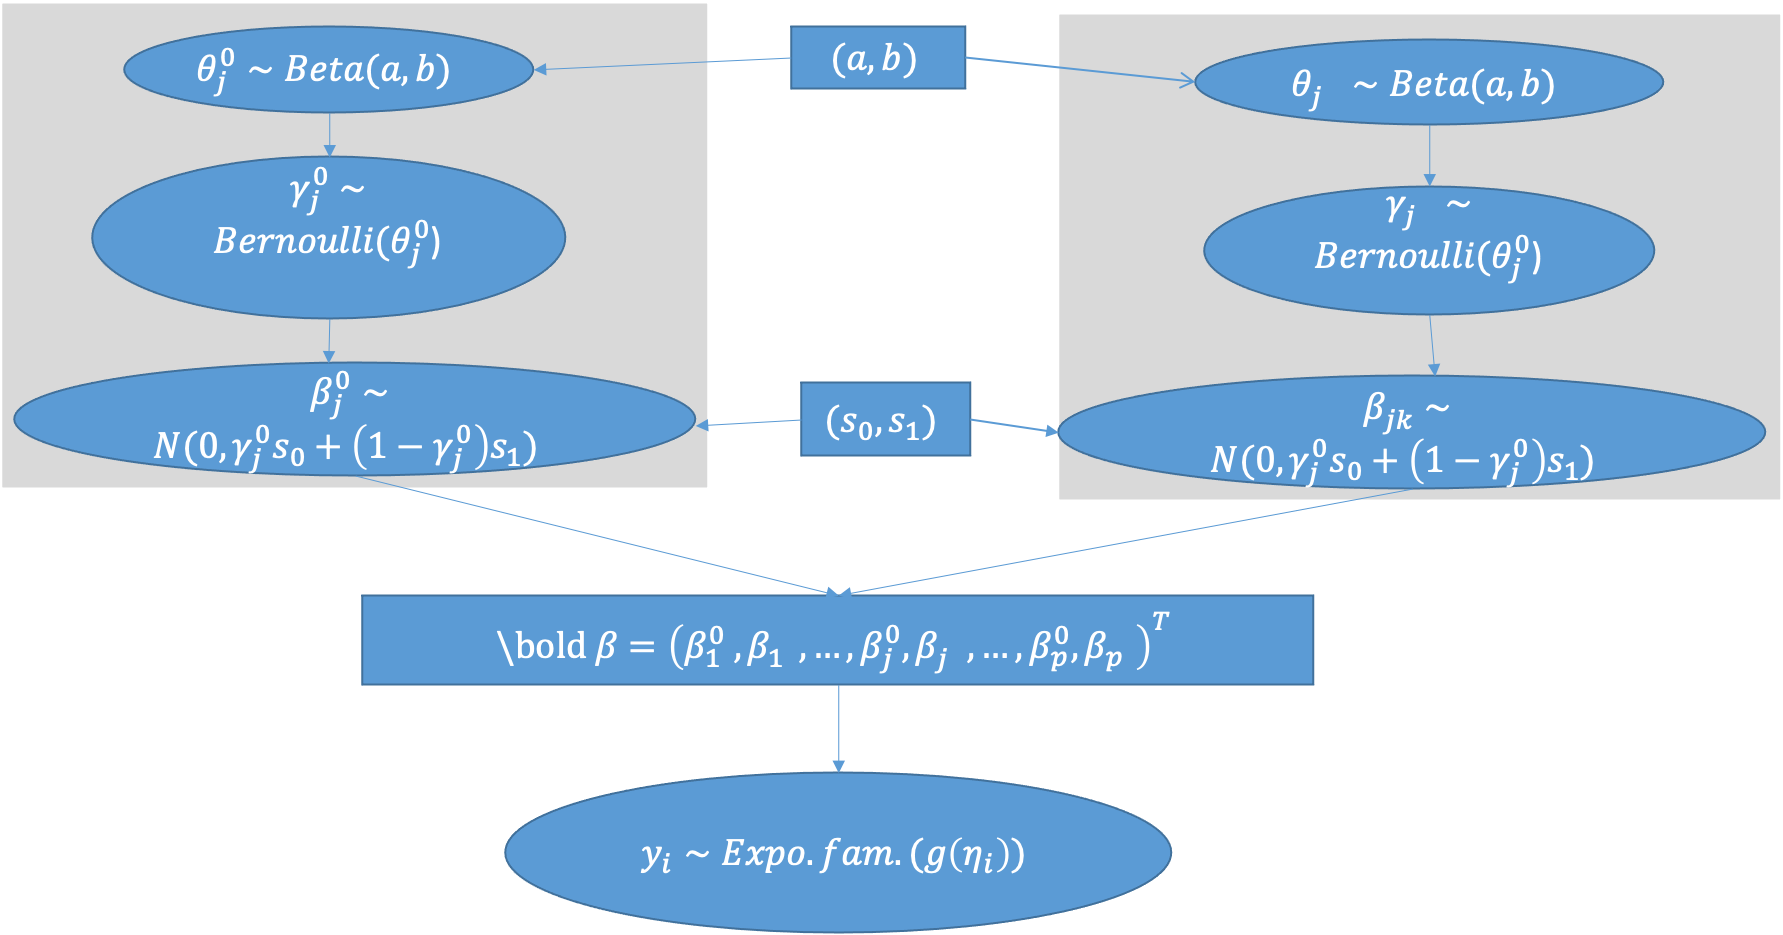
\includegraphics{Fig/SS_prior_flow_chart.png}

~

\hypertarget{mixture-double-exponential-prior}{%
\subsubsection{Mixture Double Exponential
Prior}\label{mixture-double-exponential-prior}}

One of the critics received by the spike-and-slab mixture normal prior
is that the tails of a normal distribution diminishes to zero too fast,
which renders problem when estimating the large effects. In contrast,
distributions with heavier tails are preferred, for example \(t\)
distribution with small degree of freedom and double exponential
distribution. Specifically, double exponential prior is equivalent to
the LASSO penalty in the frequentist models, providing a sparse
solution. Meanwhile, the estimation algorithm of LASSO penalty are
extremely efficient, greatly reducing the computation needs. Recent
developments of spike-and-slab priors include spike-and-slab LASSO
prior, i.e.~spike-and-slab mixture double exponential prior. We extend
the spike-and-slab LASSO prior to high-dimensional GAMs, providing
computationally efficiency and sparse solution to our proposed ssGAM-MN.

The set-up of ssGAM-LASSO model is similar to ssGAM-MN, except we
replace the normal distribution with double exponential distribution.
The prior distributions of the coefficients \(\beta^0_j, \beta^{pen}_j\)
for the \(j\) predictor can be formulated as \[
\begin{aligned}
  \beta^0_{j} |\gamma^0_{j},s_0,s_1 &\sim DE(0,(1-\gamma^0_{j}) s_0 + \gamma^0_{j} s_1)\\
  \beta^{pen}_{jk} | \gamma^{pen}_{j},s_0,s_1 &\sim DE(0,(1-\gamma^{pen}_{j}) s_0 + \gamma^{pen}_{j} s_1).
\end{aligned}
\] The hyper-priors for \(\gamma^0_j, \gamma^{pen}_j, \theta_j\) are
kept the same as specified in ssGAM-MN.

\hfill\break

\hypertarget{alforithm-for-fitting-ssgams}{%
\subsection{Alforithm for fitting
ssGAMs}\label{alforithm-for-fitting-ssgams}}

Parsimonious computation is always encouraged in high-dimension data
analysis. Normally, Bayesian methodology loses its advantages over
Frequentest penalized model because of the computation cost. Previous
Bayesian spline models heavily relies on the MCMC algorithm to establish
posterior distribution of parameters. One of the exception is Bai (in
progress), who a grouped spike-and-slab LASSO prior \citep{Rockova2018}
to address the grouping structure of spline bases. He focused on the MAP
estimator of the parameters, but failed to address the uncertainty
measure of the estimates. The main difference between Bai's work and the
proposed models are two-folded: 1) the proposed models are feasible to
answer the question if the non-linear effects are necessary for the
predictors, while Bai's work can't due to the ``all-in-all-out''
approach; 2) the proposed models can provide uncertainly measures in
addition to the point estimates of the coefficients, while Bai's work
can't not due to the model fitting algorithm.

In the follow section, we introduced two expectation-maximization (EM)
based algorithms for fast computing, EM-IRLS and EM-coordinate Descent
algorithm. Instead of simulating the posterior distribution via MCMC, we
iteratively estimate the MAP. Compared to the EM-IRLS algorithm, the
EM-coordinate descent provides an expedited model fitting process at the
cost of model uncertainty.

\hfill\break

\hypertarget{em-algorithms}{%
\subsubsection{EM algorithms}\label{em-algorithms}}

EM algorithm is an iterative algorithm to find the maximum likelihood
estimates or the Bayesian counterpart MAP estimates. It is commonly used
when some necessary data to establish the likelihood function are
missing. Instead, the algorithm maximizes the expectation, in respect to
the ``missing'' data, of the likelihood function.

The recursive algorithm consists of two steps:

\begin{itemize}
\tightlist
\item
  E-step: to calculate the expectation of the likelihood function
  conditioning on some ``missing'' data
\item
  M-step: to maximize the spectated likelihood function to calculate the
  parameter of interest
\end{itemize}

For ssGAM, we define the parameters of interest as
\(\Theta = {\boldsymbol{\beta}, \boldsymbol{\theta}, \phi}\) and
consider the latent binary indicators \(\boldsymbol{\gamma}\) as
nuisance parameters of the model. Our objective is to find the
parameters \(\Theta\) that maximize the posterior density function,or
equivalently, the logarithm of the density function, \[
\begin{aligned}
& \text{argmax}_{\Theta}
\log p(\Theta, \boldsymbol{\gamma}| \textbf{y}, \textbf{X}) \\
&= \log p(\textbf{y}|\boldsymbol{\beta}, \phi) + \log p(\phi) + \sum\limits_{j=1}^p\left[\log p(\beta^0_j|\gamma^0_j)+\sum\limits_{k=1}^{K_j} \log p(\beta^{pen}_{jk}|\gamma^{pen}_{jk})\right]\\
& +\sum\limits_{j=1}^{p} \left[ (\gamma^0_j+\gamma_{j}^{pen})\log \theta_j + (2-\gamma^0_j-\gamma_{j}^{pen}) \log (1-\theta_j)\right] +  \sum\limits_{j=1}^{p}\log p(\theta_j)
\end{aligned}
\]\\

We use the EM algorithm to find the MAP estimate of \(\Theta\). Since
the latent binary indicators \(\boldsymbol{\gamma}\) are not of our
primary interest, we treat them as as the ``missing data'' in the EM
algorithms. Naturally In the E-step, we calculate the expectation of
posterior density function of
\(\log p(\Theta, \boldsymbol{\gamma}| \textbf{y}, \textbf{X})\) with
respect to the latent indicators \(\boldsymbol{\gamma}\) conditioning on
the values from previous iteration \(\Theta^{t-1}\), \[
E_{\boldsymbol{\gamma}|\Theta^{t-1}}\log p(\Theta, \boldsymbol{\gamma}| \textbf{y}, \textbf{X}) .
\] Hereafter, we use the short hand notation
\(E(\cdot)\equiv E_{\boldsymbol{\gamma}|\Theta^{t-1}}(\cdot)\). In the
M-step, we find the \(\Theta^{t}\) that maximize
\(E_{\boldsymbol{\gamma}|\Theta^{t-1}}\log p(\Theta, \boldsymbol{\gamma}| \textbf{y}, \textbf{X})\).
To note here, the log-posterior of ssGAM (up to additive constants) can
be written as a two-part equation

\[ \log p(\Theta, \boldsymbol{\gamma}| \textbf{y}, \textbf{X}) = Q_1(\beta, \phi) + Q_2 (\gamma,\theta),\]
Where
\[ Q_1(\boldsymbol{\beta}, \phi) = \log p(\textbf{y}|\boldsymbol{\beta}, \phi) + \log p(\phi) + \sum\limits_{j=1}^p\left[\log p(\beta^0_j|\gamma^0_j)+\sum\limits_{k=1}^{K_j} \log p(\beta^{pen}_{jk}|\gamma^{pen}_{jk})\right]\]
and \[
Q_2(\boldsymbol{\gamma},\boldsymbol{\theta}) = \sum\limits_{j=1}^{p} \left[ (\gamma^0_j+\gamma_{j}^{pen})\log \theta_j + (2-\gamma^0_j-\gamma_{j}^{pen}) \log (1-\theta_j)\right] +  \sum\limits_{j=1}^{p}\log p(\theta_j) .\]
\(Q_1\) and \(Q_2\) are respectively, the log-likelihood of model
coefficients and the dispersion parameter \(\boldsymbol{\beta}, \phi\),
and latent indicators \(\boldsymbol{\gamma}, \theta\). Conditioning on
\(\gamma_{jk}\), \(Q_1\) and \(Q_2\) are independent and can be
maximized separately for \(\boldsymbol{\beta}, \phi\) and
\(\boldsymbol{\theta}\).

The E- and M- steps are iterated until the algorithm converge. Depending
on the choice of the mixture priors, either mixture normal or mixture
double exponential, the maximization in the M-step can take different
algorithms, IRLS for uncertainty measures and coordinate descent for
faster computation.

\hfill\break

\hypertarget{em-irls}{%
\subsubsection{EM-IRLS}\label{em-irls}}

The main idea of the EM-IRLS algorithm is to use the iterative
re-weighted least square algorithm to find the estimate
\(\boldsymbol{\beta}, \phi\) that maximizes \(E(Q_1)\). Recall the prior
set-up of mixture normal prior, we have the prior densities of
\(\boldsymbol{\beta}\) conditioning on \(\boldsymbol{\gamma}\)

\[
\begin{aligned}
p(\boldsymbol{\beta }| \boldsymbol{\gamma}) &\propto \prod\limits_{j=1}^{p}\left[{S^0_j}^{-1/2}\exp(-1/2({\beta^0_{j}}^2/S^0_{j}))\prod\limits_{k=1}^{K_j}S_{j}^{-1/2}\exp(-1/2(\beta_{jk}^2/S_{j}))\right],%\\
% p(\bs\gamma | \bs \theta) & = \prod\limits_{j=1}^{p}\prod\limits_{k=1}^{K_j} \theta_j^{\gamma_{jk}} (1-\theta_j)^{1-\gamma_{jk}}.
\end{aligned}
\] and \begin{align*}
E(Q_1) &= \log p(\textbf{y}|\boldsymbol{\beta}, \phi) + \log p(\phi) + \sum\limits_{j=1}^{p} \left[E({S^0_j}^{-1}){\beta^0_j}^2+\sum\limits_{k=1}^{K_j}E(S^{-1}_{j})\beta_{jk}^2\right]\\
E(Q_2) &= \sum\limits_{j=1}^{p}\sum\limits_{k=1}^{K_j} \left[ E(\gamma_{jk})\log \theta_j + (1-E(\gamma_{jk})) \log (1-\theta_j)\right] +  \sum\limits_{j=1}^{p}\log p(\theta_j)
\end{align*} where
\(S_{j}^0 = (1-\gamma^{0}_{j}) s_0 + \gamma^{0}_{j} s_1\) and
\(S_{j} = (1-\gamma^{pen}_{j}) s_0 + \gamma^{pen}_{j} s_1\). To
calculate two unknown quantities \(E({S_j^0}^{-1})\) and
\(E(S^{-1}_j)\), the posterior probability
\(p^0_{j} \equiv p(\gamma^{0}_{j}=1|\Theta^{t-1})\) and
\(p_{j} \equiv p(\gamma^{pen}_{j}=1|\Theta^{t-1})\) are necessary, which
can be derived via Bayes' theorem. The calculation for \(p_j\) is
slightly different from that of \(p^0_j\), as \(p_j\) depends on the
value of \(\beta_{jk}\) for \(k=1, \dots, K_j\) and \(p^0_j\) only
depends on \(\beta_j^0\). The calculation follows the equations below.

\[
\begin{aligned}
p_{j}^0 &= \frac{Pr(\gamma_{j}^0 = 1|\theta_j)f(\beta_{j}^0|\gamma_{j}^0=1, s_1) }{Pr(\gamma_{j}^0 = 1|\theta_j)f(\beta_{j}^0|\gamma_{j}^0=1, s_1) + Pr(\gamma_{j}^0 = 0|\theta_j)f(\beta^0_{j}|\gamma^0_{j}=0, s_0)}\\
p_{j} &= \frac{Pr(\gamma^{pen}_{j} = 1|\theta_j)\prod\limits_{k=1}^{K_j}f(\beta_{jk}|\gamma^{pen}_{j}=1, s_1) }{Pr(\gamma^{pen}_{j} = 1|\theta_j)\prod\limits_{k=1}^{K_j}f(\beta_{jk}|\gamma^{pen}_{j}=1, s_1) + Pr(\gamma^{pen}_{j} = 0|\theta_j)\prod\limits_{k=1}^{K_j}f(\beta_{jk}|\gamma^{pen}_{j}=0, s_0)}
\end{aligned}
\]

and
\(Pr(\gamma_{j}^{0} = 1|\theta_j) =Pr(\gamma_{j}^{pen} = 1|\theta_j) = \theta_j\),
\(Pr(\gamma_{j}^{0} = 0|\theta_j) = Pr(\gamma_{j}^{pen} = 0|\theta_j) = 1-\theta_j\),
\(f(\beta|\gamma=1, s_1) = \text{Normal}(\beta|0 , s_1)\),
\(f(\beta|\gamma=0, s_0) = \text{Normal}(\beta|0 , s_0)\). It is trivial
to show \[
\begin{aligned}
&E(\gamma^0_{j})  = p^0_{j} & &E(\gamma^{pen}_{j})  = p_{j}\\
&E({S^0}^{-1}_{j}) = \frac{1-p^{0}_{j}}{s_0} + \frac{p^{0}_{j}}{s_1} & &E(S^{-1}_{j}) = \frac{1-p_{j}}{s_0} + \frac{p_{j}}{s_1}.
\end{aligned}
\]

With \(E({S^0}^{-1}_{j})\) and \(E(S^{-1}_{j})\) known, \(E(Q_1)\) can
be also viewed as a \(l_2\) penalized likelihood function:
\(E({S^0}^{-1}_{j})\) controls the shrinkage of the linear effect,
informing if the predictor should be included in the model;
\(E(S^{-1}_{j})\) controls the smoothness of the spline function.
\(l_2\) penalized likelihood function can be maximize using the IWLS
algorithm. The likelihood function can be approximate by a weighted
normal likelihood: \[
  p(\textbf{y}|\boldsymbol{\beta}, \phi) \approx Normal(\textbf{z}|X\beta, \phi\Sigma)
\] where the `normal response' \(z_i\) and `weight' \(w_i\) are called
the pseudo-response and pseudo-weight, respectively.The pseudo data and
the pseudo-weight are calculated by \[
    \begin{aligned}
    z_i &= \hat\eta_i - \frac{L^{'}((y_i|\hat\eta_i))}{L^{''}((y_i|\hat\eta_i))}& w_i &= - L^{''}((y_i|\hat\eta_i)),
    \end{aligned}
    \] where \(\eta_i = \sum\limits_{j=1}^p \hat f_j^{(t)}(x_{ij})\) is
the estimated linear predictor using current estimated value of
\(\boldsymbol{\beta}\), \(L^{'}\) and \(L^{''}\) are the first
derivative and second derivative of the log-likelihood function. The
\(l_2\) penalty,
\(\sum\limits_{j=1}^{p}\left[E({S^0_j}^{-1}){\beta^0_j}^2+\sum\limits_{k=1}^{K_j}E(S^{-1}_{j})\beta_{jk}^2\right]\)
can be seems as a multivariate normal distribution of mean
\(\textbf{0}\) and variance-covariance matrix
\(\Sigma(E({S^0}_1^{-1}), E(S_1^{-1}), \dots, E({S_p^0}^{-1}), E(S_p^{-1})\),
conditioning on the value of \(E({S^0_1}^{-1}), \dots E({S^0_p}^{-1})\).
An augmentation step combines the normal approximation and multivariate
normal for \(\boldsymbol{\beta}\), similarly to Ridge regression model
fitting. The estimates of \(\boldsymbol{\beta}\) and \(\phi\) can be
quickly updated in the IRLS algorithm.

The remaining parameters of interest \(\boldsymbol{\theta}\) can be
updated by maximizing \(E(Q_2)\). As the beta distribution is a
conjugate prior for Bernoulli distribution, \(\boldsymbol{\theta}\) can
be easily updated with a closed form equation: \[
\theta_j = \frac{p^0_j + p_{j} + a - 1 }{a + b}.
\]

Totally, the framework of the proposed EM IRLS algorithm was summarized
as follows:

\begin{enumerate}
\def\labelenumi{\arabic{enumi})}
\item
  Choose a starting value \(\boldsymbol{\beta}^{(0)}\) and
  \(\boldsymbol{\theta}^{(0)}\) for \(\boldsymbol{\beta}\) and
  \(\boldsymbol{\theta}\). For example, we can initialize
  \(\boldsymbol{\beta}^{(0)} = \boldsymbol{0}\) and
  \(\boldsymbol{\theta}^{(0)} = \boldsymbol{0}.5\)
\item
  Iterate over the E-step and M-step until convergence
\end{enumerate}

E-step: calculate \(E(\gamma^0_{j})\), \(E(\gamma^{pen}_{j})\)and
\(E({S^0}^{-1}_{j})\) , \(E({S}^{-1}_{j})\)with estimates of
\(\Theta^{(t-1)}\) from previous iteration

M-step:

\begin{enumerate}
\def\labelenumi{\alph{enumi})}
\item
  Update \(\boldsymbol{\beta}^{(t)}\) using the IRLS algorithm
\item
  Update \(\boldsymbol{\theta}^{(t)}\) using the closed form equation
\end{enumerate}

We assess convergence by the criterion:
\(|d^{(t)}-d^{(t-1)}|/(0.1+|d^{(t)}|)<\epsilon\), where
\(d^{(t)} = -2l(\beta^{(t)},\phi^{(t)})\) is the estimate of deviance at
the \(t\)th iteration, and \(\epsilon\) is a small value (say
\(10^{-5}\)).

\hfill\break

\hypertarget{em-coordinate-descent}{%
\subsubsection{EM-Coordinate Descent}\label{em-coordinate-descent}}

When the prior distribution is set to mixture double exponential,
coordinate descent algorithm can be used to estimate
\(\boldsymbol{b}eta\), replacing IRLS, in the M-step. Coordinate descent
is an optimization algorithm that offers extreme computational
advantage, and famous for its application in optimizing the \(l_1\)
penalized likelihood function.

Recall, the density function of spike-and-slab mixture double
exponential prior can be written as \[
f(\beta|\gamma, s_0, s_1) = \frac{1}{(1-\gamma)s_0 + \gamma s_1}\exp(-\frac{|\beta|}{(1-\gamma)s_0 + \gamma s_1}).
\]

This can simplify our posterior likelihood function to \[
E(Q_1) = \log p(\textbf{y}|\boldsymbol{\beta}, \phi) + \log p(\phi) + \sum\limits_{j=1}^p\left[E({S^0_j}^{-1})|\beta^0_j|+\sum\limits_{k=1}^{K_j}E(S^{-1}_{j})|\beta_{jk}|\right]
,
\] where the approximation of \(E({S^0_j}^{-1}\) and \(E(S^{-1}_{j})\)
remains the same as in the EM-IRLS algorithm. The formulation of
\(E(Q_1)\) can be seen as a \(l_1\) penalized likelihood function, and
optimized via coordinate descent algorithm. The estimates can be used to
further estimates \(\boldsymbol{\theta}\) in the M-step, following the
same equation in the EM-IRLS.

Totally, the framework of the proposed EM-coordinate descent algorithm
was summarized as follows:

\begin{enumerate}
\def\labelenumi{\arabic{enumi})}
\item
  Choose a starting value \(\boldsymbol{\beta}^{(0)}\) and
  \(\boldsymbol{\theta}^{(0)}\) for \(\boldsymbol{\beta}\) and
  \(\boldsymbol{\theta}\). For example, we can initialize
  \(\boldsymbol{\beta}^{(0)} = \boldsymbol{0}\) and
  \(\boldsymbol{\theta}^{(0)} = \boldsymbol{0}.5\)
\item
  Iterate over the E-step and M-step until convergence
\end{enumerate}

E-step: calculate \(E(\gamma^0_{j})\), \(E(\gamma^{pen}_{j})\)and
\(E({S^0}^{-1}_{j})\) , \(E({S}^{-1}_{j})\)with estimates of
\(\Theta^{(t-1)}\) from previous iteration

M-step:

\begin{enumerate}
\def\labelenumi{\alph{enumi})}
\item
  Update \(\boldsymbol{\beta}^{(t)}\) using the coordinate descent
  algorithm
\item
  Update \(\boldsymbol{\theta}^{(t)}\) using the closed form equation
\end{enumerate}

We assess convergence by the criterion:
\(|d^{(t)}-d^{(t-1)}|/(0.1+|d^{(t)}|)<\epsilon\), where
\(d^{(t)} = -2l(\beta^{(t)},\phi^{(t)})\) is the estimate of deviance at
the \(t\)th iteration, and \(\epsilon\) is a small value (say
\(10^{-5}\)).

~

\hypertarget{selecting-optimal-scale-values}{%
\subsection{Selecting Optimal Scale
Values}\label{selecting-optimal-scale-values}}

Our proposed prior, spike and slab spline prior, requires two preset
scale parameters (\(s_0\), \(s_1\)). Hence, we would construct a two
dimensional grid, consists of different pairs of (\(s_0\), \(s_1\))
value. However, previous research on the topic\footnote{TODO: add
  citation} suggested the value of slab scale \(s_1\) have less impact
on the final model and is recommended to be set as a generally large
value of \(s_1 = 1\) that provides no or weak shrinkage. More attention
is focused on examining different values of spike scale \(s_0\). Instead
of the 2-D grid, We consider a sequence of \(L\) decreasing values
\(\{s_0^l\}: 0 < s_0^1 < s_0^2 < \dots < s_0^L < s_1\). Increasing the
spike scale s\_0 tends to include more non-zero coefficients in the
model. An measure of preference, e.g.~area under the curve (AUC), mean
squared error, can be used to facilitate the selection of a final model.
The procedure is similar to the lasso implemented in the widely used R
package \texttt{glmnet}, which quickly fits the lasso model over a list
of values of \(\lambda\) covering the entire range, giving a sequence of
models for users to choose from.

\hypertarget{simulation-study}{%
\subsection{Simulation Study}\label{simulation-study}}

In this section, we compare the performance of the proposed models to 3
other models: COSSO, adaptive COSSO ,mgcv. COSSO is xxx method. Adaptive
COSSO is another method, mgcv is another method. To demonstrate the
correctness and feasibility of the proposed SS-GAM, we follow the
logistic regression simulation introduced in Bai (Work in Progress). We
first generate \(n=500\) training data sample with number of predictors
\(p=4, 10, 50, 200\) respectively, where the predictors
\(X \sim MVN_{n\times p}(0, I_{P})\). We simulate the outcome data from
three distributions, gaussian, poisson, and binomial with the identity
link, logit link \(g(x) = \log(\frac{x}{1-x})\), and log link
\(g(x) = log(x)\) functions to mimic the common use of generalized
model. The outcome is simulated via the following function \[
\mathbb{E}(Y) = g^{-1}(5 \sin(2\pi x_1) - 4 \cos(2\pi x_2 -0.5) + 6(x_3-0.5) - 5(x_4^2 -0.3))
\] for gaussian and binomial outcome and shrinked effects

\[
\mathbb{E}(Y) = g^{-1}(\sin(2\pi x_1) - 2\cos(2\pi x_2 -0.5) + 0.4(x_3-0.5) - 2(x_4^2 -0.3))
\] for stable poisson outcome. For the Gaussian outcome where dispersion
are required, the dispersion parameter was set to 1. We follow the same
data generating functions in Bai. In this data generating process, we
have \(x_1, x_2, x_3, x_4\) as the active covariates, while the rest
covariates are inactive \(f_j(x_j) = 0\) for \(j = 4, \dots, p\).
Another set of independent sample of size
\(n_{test}=1000\),(\(x_{new} ,y_{new}\)), are created following the same
data generating process, serving as the testing data. For mgcv and
proposed models where choice of spline function are customizable, we
choose to cubic regression spline with 10 basis. In COSSO and adaptive
COSSO where the choice of spline are pre-determined, we set to have 10
bases. The corresponding number of parameter that we estimate with the
model is 37, 82, 451 and 1801. We are run the simulation where the
number of bases are increased to 25 deliberately. To evaluate the
performance of the models, mean squared error, mean absolute error for
gaussian model, AUC and misclassifcation rate are calculated for
binomial model, and deviance are calculated for Poisson model, averaging
across50 simulations. The results are tabulated in Table 1, 2, 3.

\%are calculated to assess out-of-sample estimation accuracy,

\%We also calculated the area under the curve (AUC) of the receiver
operating characteristic curve for \(y_{new}\). We will also visually
display the estimated smooth function with the smooth function of truth
to compare if the models can infer the smooth function correctly,
despite the prediction accuracy.

\%When constructing the smooth function of each variables, we constructs
the natural cubic spline with degree of freedom 25. In other words, the
design matrix of each smooth function will have 26 columns. The total
number of columns for \(p=4, 10, 50\) is \(105, 261, 1301\)
respectively, where intercept is kept in the model when fitting. The
\(p=50\) can mimic the high dimensional setting as the design matrix are
in high-dimensional setting (\(p >> n\))

\%We benchmark the performance of the proposed methods with the state of
art GAM package \texttt{mgcv}{[}TODO: add citation{]}. In the future
steps, we will compare our proposed model with other high dimensional
GAM applications.

~

\hypertarget{simulation-results}{%
\subsubsection{Simulation Results}\label{simulation-results}}

Overall, the proposed priors outperforms the state-of-art GAM model
\texttt{mgcv} when the dimensionality is low, median, and high. The
proposed priors predicts better than \texttt{mgcv} and infers better of
the underlying smooth function. Most importantly, \texttt{mgcv} is
infeasible in the high dimensional setting, i.e.~when \(p=50\) where the
number of parameters are greater than the sample size.

\hypertarget{prediction-performace}{%
\paragraph{Prediction Performace}\label{prediction-performace}}

The prediction performance is tabulated in the table below for AUC and
Supplementary tables for MSE and misclassification rate. In summary, the
proposed Bayesian models outperforms the benchmark model \texttt{mgcv}
regardless the choice of prior or fitting algorithm. The models with
IRLS fitting algorithm give slightly better performance than the the
model with cyclic coordinate descent algorithm. The advantage diminishes
in the high dimensional setting (p=50). This is possible because the SS
normal spline prior provides a more smooth solution, which would work
well in a low to median dimension setting. However, in the high
dimensional setting, there are not enough sparsity in the model, i.e.~SS
normal prior will provides a more complex model than necessary. This is
confirmed with the visualization in the following section.

\hypertarget{visualization}{%
\paragraph{Visualization}\label{visualization}}

We plot the estimated smooth functions of the four active variables for
the 100 simulation iterations, along with the `true' smooth function.
Across different settings of predictors, the patterns look similar.
First of all, in all the settings, \texttt{mgcv} tends to provide more
extreme models, where in the graphs the smooth function have much higher
bound than the true smooth function. Rarely the estimated smooth
function from \texttt{mgcv} matches with the true smooth function. In
comparison, the proposed method can interpolate the shape of the true
smooth function. However, different priors and fitting algorithms have
different advantages. For example, in Figure 1, we see that the SS
normal distribution have problem with the tail of the smooth function,
especially obvious in the estimations of the variable \emph{x4}.
However, it would have less sparse solutions, which is more likely to
accurately interpolate the smooth function especially when the shape is
complicated (see variable \emph{x2}). On the contrary, the SS double
exponential prior model encourages sparse solutions, which can sometime
omit active predictors.

\hypertarget{real-data-analysis}{%
\section{Real Data Analysis}\label{real-data-analysis}}

\hypertarget{discussion}{%
\section{Discussion}\label{discussion}}

Remaining issue: 1. Degree of freedom has yet to closely studied. As an
direct impact, the functional selection can be improved when effective
degree of freedom are more carefully studied 2. While the proposed model
addresses a great deal of analytic problem, analyzing the time-to-event
outcome remains unsolved. Our current effort resides on expanding. An
naive approach could be convert an time-to-event outcome to a poisson
outcome following xxx. Hence, the . However, it would be more efficient
to , via penalized pseudo likelihood function, which is the current
effort resides. 2. Future exapansion, as we were analyzing the
metabolites data, we observed that metabolites pathway infromation can
be useful in the predictive and integrative model can be developed based
on the proposed framework. As an naive solution, the selection indicator
of linear effect of the spline terms of all metabolites on the same
pathway can be set to share the same hyper prior such that the group
selection can be modestly achieved. Meanwhile further advancedment of
the methodology regarding to the integrative analysis can consider
setting the hypor priors of the selection indivator of the non-linear
components conditioning on the probability of inclusion of the linear
effect. Such structure is more sensible analytically.

\hypertarget{discussion-1}{%
\subsection{Discussion}\label{discussion-1}}

In this chapter, we propose the spike-and-slab generalized additive
models for high-dimensional analysis.Two fast computing algorithms,
EM-IRLS and EM-coordinate descent are developed for expedited model
fitting. EM-IRLS provides uncertainty measures, while EM-coordinate
descent algorithm are extremely fast for model fitting. In the
simulation studies, we shows the proposed model outperforms the state of
the art GAM model, \texttt{mgcv} in prediction and function inference.
Moreover, due to the model selection nature of the spike-and-slab prior,
the proposed model can identify predictors that have large effects on
the outcome. In addition, the model can be used to answer the question
if non-linear effect are necessary.

In the manuscript, we describe the implementation of ssGAM-NM using
EM-IRLS. Nevertheless, EM-IRLS are not limited to fitting ssGAM-NM.
Other spike-and-slab prior can be fitted with EM-IRLS as well,
e.g.~mixture t-distribution, and mixture double exponential
distributions. \citet{Yi2012} demonstrated that t prior and double
exponential prior can be seen hierarchical normal priors, \[
\begin{aligned}
\beta_i \sim N(0, \tau^2_i),\\
\tau^2_i \sim Inv-\chi^2(v, s^2_j) \text{ or } \tau^2_i \sim Gamma(1, s^2/2)
\end{aligned}
\] with \(\tau^2\) integrated out analytically. Hence, the EM-IRLS can
be easily applied to those two additional mixture priors. One of the
advantage of using mixture \(t\) prior over mixture normal prior is that
\(t\) distributions with low degree of freedom, e.g.~\(v=1\), have
heavier tail than the normal distribution, which is also a special case
of \(t\) distribution when \(v=\infty\). The heavier tails help to
obtain posteriors that concentrated around the true nonzero coefficients
at optimal rates. \citep{Rockova2014a}

\ldots and can be referenced (Figure \ref{fig:plot}) by including the
\texttt{\textbackslash{}\textbackslash{}label\{\}} tag in the
\texttt{fig.cap} attribute of the R chunk:
\texttt{fig.cap\ =\ "Fancy\ Caption\textbackslash{}\textbackslash{}label\{fig:plot\}"}.
It is a quirky hack at the moment, see
\href{https://github.com/yihui/knitr/issues/323}{here}.

Analogously, use Rmarkdown to produce tables as usual:

\hypertarget{cross-referencing}{%
\subsection{Cross-referencing}\label{cross-referencing}}

The use of the Rmarkdown equivalent of the \LaTeX cross-reference system
for figures, tables, equations, etc., is encouraged (using
\texttt{{[}@\textless{}name\textgreater{}{]}}, equivalent of
\texttt{\textbackslash{}ref\{\textless{}name\textgreater{}\}} and
\texttt{\textbackslash{}label\{\textless{}name\textgreater{}\}}). That
works well for citations in Rmarkdown, not so well for figures and
tables. In that case, it is possible to revert to standard
\LaTeX syntax.

\hypertarget{references}{%
\section{References}\label{references}}

\bibliography{bibfile.bib}


\end{document}
